\section{Introduction}
\label{sec:intro}

\begin{figure*}[t]
  \centering
  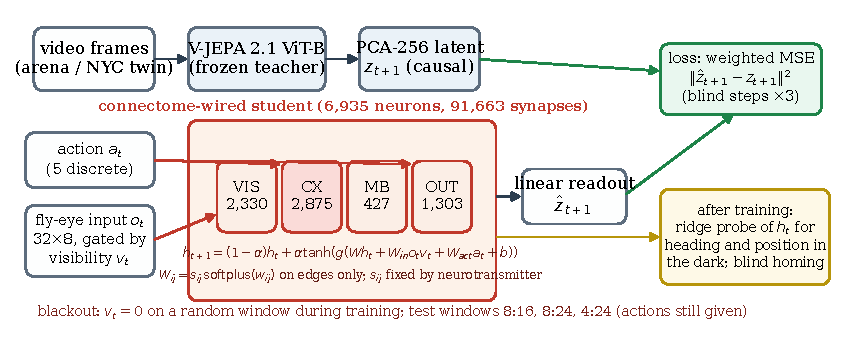
\includegraphics[width=\linewidth]{fig/schematic.pdf}
  \caption{\textbf{A video world model, distilled into a fly's wiring diagram.} A frozen \vjepa encoder turns each frame
  of an episode into a causal latent $z_t$. The student is a leaky rate network whose recurrence $W$ lives only on the
  91,663 signed synapses of the \flywire connectome (VIS, CX, MB and OUT populations); training can scale a synapse but
  never flip its sign or add one. The single training signal is next-latent prediction, with the visual input randomly
  cut (``blackout'') so that the state must carry the latent forward from the action record alone. Everything we
  report about heading, position and homing is read out of the trained state afterwards; none of it was supervised.}
  \label{fig:schematic}
\end{figure*}

Ask a world model to imagine the next second of a video and it will do a reasonable job. Ask it what it imagines after
the lights go out, and the answer depends entirely on what its recurrent core chose to remember. In most video world
models that core is a generic block, a GRU or a transformer layer, sized by compute budget and trained with nothing
but the prediction loss to guide what it keeps~\cite{ha2018world,hafner2023dreamerv3,assran2025vjepa2}. Biology took a
different route to the same problem. A fruit fly in darkness holds its heading and a vector back to where it started
for many seconds, using a few thousand neurons of its central complex, and the complete synapse-level wiring of that
circuit is now public~\cite{seelig2015neural,green2017neural,turnerevans2017angular,dorkenwald2024neuronal,schlegel2024whole}.

This paper puts the two together and asks a plain question: \emph{if a world model's recurrence is forced to be the
fly's wiring diagram, what does the wiring buy?} We distil \vjepa~\cite{assran2025vjepa2}, a self-supervised video
foundation model, into a leaky rate network of 6,935 \flywire neurons whose only recurrent weights sit on the 91,663
signed synapses of the real connectome (\cref{fig:schematic}). The student never sees the teacher's weights, only its
latent through the loss. It is trained on one objective, next-latent prediction under random blackouts of the visual
input, so any structure that appears in its state was not asked for.

\begin{figure*}[t]
  \centering
  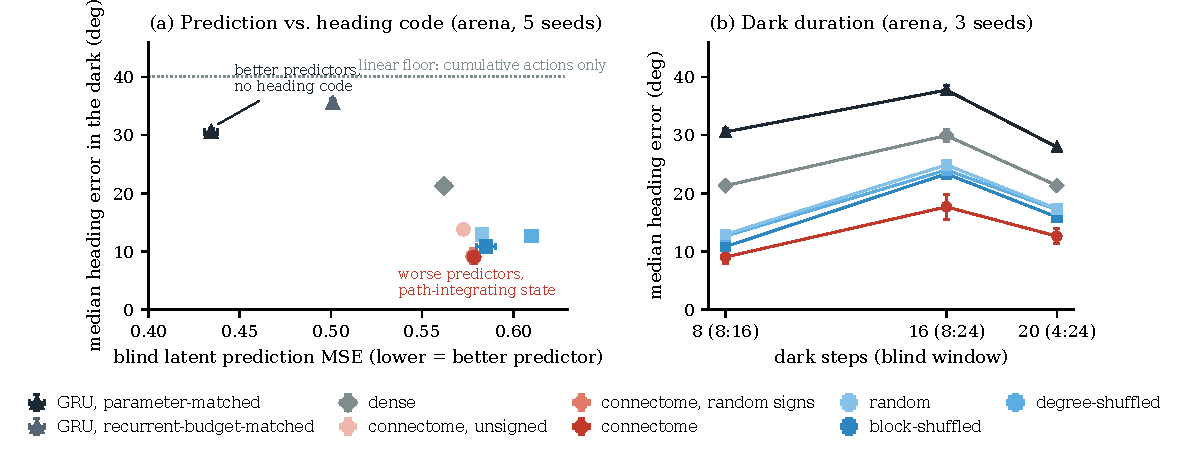
\includegraphics[width=\linewidth]{fig/main_result.pdf}
  \caption{\textbf{The wiring makes a worse predictor and a better integrator.} (a) Each point is one wiring (mean\pm sd
  over 5 seeds): blind latent-prediction error on the $x$-axis, median heading error decoded from the state during 8
  dark steps on the $y$-axis. Both GRUs predict the teacher best and keep almost no heading; the connectome and its
  sparse controls predict worse and keep heading to about 10\degree. A linear readout of the cumulative actions alone
  gives 40\degree\ (dotted). (b) The code degrades gracefully with the length of the dark window, and the real
  wiring's margin over block-shuffled grows from 2\degree\ to 6\degree\ at 16 dark steps.}
  \label{fig:main}
\end{figure*}

The answer has two halves, and we think both are worth stating plainly. The wiring is \emph{not} a better predictor.
Against controls that hold neuron count, edge count, region block structure, Dale's-law sign structure and parameter
count fixed, the real connectome beats its shuffled twins by about one percent of latent error, consistently, while a
parameter-matched GRU is 25\,\% better and a GRU matched to the connectome's \emph{recurrent} budget is still 13\,\%
better. What the wiring buys instead is a \emph{path-integrating state} (\cref{fig:main}). During the blind steps a
ridge probe reads heading from the connectome state to 9\degree\ median error and position to $R^2$\,0.94. The
parameter-matched GRU, which predicts the latent far better, gives 31\degree\ and 0.41; the budget-matched GRU gives
36\degree\ and 0.30; a linear readout of the action history, which is all the state could possibly have integrated,
gives 40\degree. The code survives 16 and 20 dark steps, shows up again in a city-scale raycast twin of Manhattan, and
widens rather than closes under a non-linear probe.

Three further findings keep the claim honest, and we report all of them in full. First, sparse random and
block-shuffled wirings of the same size form the code too, 2\degree\ to 6\degree\ worse than the real graph; the exact
synapse list is a small, reproducible bonus, not the cause. Second, a linear readout of the state drives blind homing
well above a random-action floor (NYC twin: 37\,\% success against 0\,\%) but well below a dead-reckoning ceiling
(92\,\%), and steering toward a decoded goal vector does not beat random actions. The controller is not the bottleneck;
the readout is. Third, on real handheld video no student, fine-tuned or not, beats a copy-last-visible baseline.

\paragraph{Contributions}
\begin{itemize}
  \item A distillation recipe that turns a video foundation model into a world model whose recurrence is a fixed,
        signed, biologically sourced sparse graph, with controls that separate wiring identity from density, degree
        sequence, region structure and sign structure (\cref{sec:method}).
  \item The first demonstration, to our knowledge, that a connectome-wired latent predictor forms a linearly readable
        heading and position code in the dark that a GRU trained on the same objective does not, with the
        information-ceiling, feature-count and non-linearity controls needed to read that result correctly
        (\cref{sec:probes}).
  \item A behavioural test of that code (blind homing, goal-vector navigation) with oracle, dead-reckoning and random
        controls, reported in full including the negative outcomes, plus cost, data efficiency, scaling, subgraph
        ablation and real-video transfer (\cref{sec:behaviour,sec:more}).
  \item Two environments (a 360\degree\ arena and a raycast twin of Midtown Manhattan), the full pipeline, and all 424
        checkpoints across 5 seeds and 12 wirings, released for reuse.
\end{itemize}
